\section{Method}
\subsection{Preprocessing}
\subsection{kNN}
KNN is a supervised. The method is non parametric meaning that the method does not make any assumption about the distribution of the data. The method is also labeled as lazy learning, as the it does not use any training points to do any generalization.\\

\begin{figure}[H]
\centering
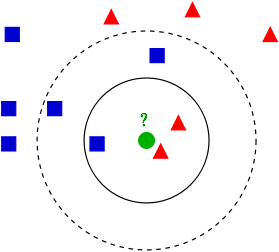
\includegraphics[width = 0.3\textwidth]{img/kNN-classification.png}
\caption{kNN classification  - the green circles has to be classified between the two classes indicated as red triangles and blue squares. k= 3}
\end{figure}

The purpose of this algorithm is to classify a new object based on its attributes and the training samples that has been used. The algorithm decides which class a new object belongs to by inspecting the k nearest neighbours, and based on the class which is the majority, will the class of the new object be determined. The number of k can be either a even or odd number, in the case of a tie with a even numbered k will the class be randomly be decided amongst the two competing ones, one have to choose the optimal value for k  in order to get an accurate predictor. The distance between two can be computed different ways, such as \\

\textbf{Euclidian distance}

\begin{equation}
d(\overrightarrow{w},\overrightarrow{v}) = \sqrt{\sum_{i}^n (w_i - v_i)^2}
\end{equation}

\textbf{Manhattan distance}

\begin{equation}
d(\overrightarrow{w},\overrightarrow{v}) = \sum_{i}^n (w_i - v_i)
\end{equation}

The advantages of using kNN is that it is simple to use, and works well on basic problems however it can be slow in for real-time prediction especially if the dataset used for training is large, as the method is a lazy learner.Another disadvantage of the method is that it does not learn anythign from the trainings data, but just stores them.  The method is not in particular robust against noisy data.    
\subsection{SVM}
Support vector machines is a supervised learning method that analyzes the data 
and tries to recognize patterns, within the classification domain.
 The standard SVM method is an binary classifier, which predicts for a given 
input which class the input belongs two. 
 Prediction is done based on the model it builds from the training session, the 
model provides a "clear gap" that provide the distinction between the first or 
the latter class. \\

Support vector machine constructs a hyperplane or set of hyperplanes in a high 
dimension. 
The hyperplane that has the largest distance to the nearest training data points 
of any class (so-called functional margin), provides the best separation,  since 
it result it a clear distinction between the classes, and lower general error.
\\

The goal in SVM is to find this hyperplane which provides the optimal separation 
of the classes by having the widest margin. 

\begin{figure}[H]
\centering
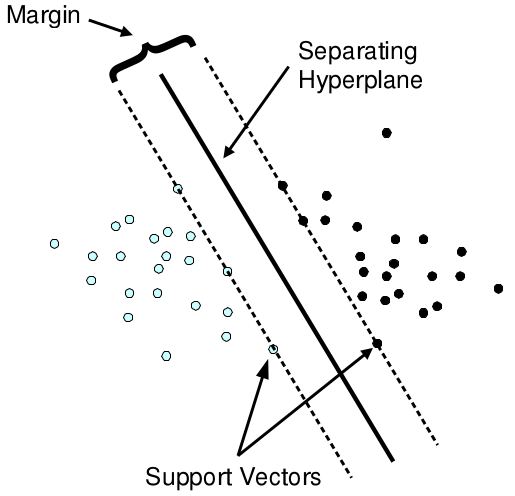
\includegraphics[width = 0.5\textwidth]{img/SVM-illu.png}
\caption{Svm Illustrated}
\label{fig::SVM-illustrated}
\end{figure}

The training data for this method consist a set of input vectors denoted as 
$\mathbf{x_i}$, each input vector has a number of component features. Each input 
vector is given a label, indicating its class.

The hyperplane is given as 
\begin{equation}
\mathbf{w} \cdot \mathbf{x} + b = 0
\end{equation}

In which the $\mathbf{w}$ determines the orientation of the plane, and 
$\mathbf{b}$ is the offset of the plane from the origin. \\
 
The seperaing hyperplane which maximizes the margin can be found by examining 
the convex hull of each class’s training data  and then find the closest points 
in the two convex hulls. The convex hull of a set of points is the
smallest convex set containing the points.  If the hyperplane that bisects both 
convex hulls can be found, will the resulting classifier deemed robust in some 
sense. 

\begin{figure}[H]
\centering
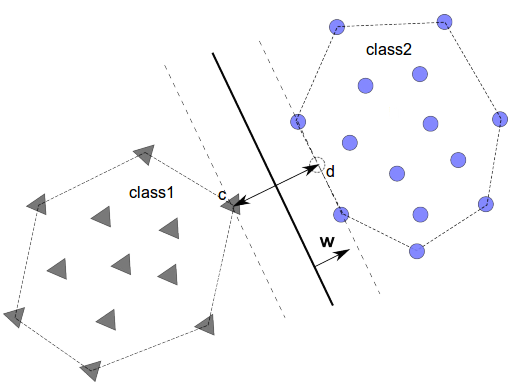
\includegraphics[width = 0.5\textwidth]{img/convex_hull.png}
\caption{Best plane bisects closest points in the convex hulls,The convex hulls 
are labeled c and d}
\label{fig::convex_hull}
\end{figure}  

To find  the plane, one have to find the points closest to the plane, which can 
be found by solving the quadratic problem. \\ 

\begin{equation}
min_\alpha~\left(\frac{1}{2} ||c-d||^2\right)
\end{equation}

where c and d are the closest to be found points, these are defined as 
\begin{equation}
\begin{aligned}
&c = \sum_{y_i~\in~class1} \alpha_ix_i  
& \text{subject to}
&& \sum_{y_i~\in~class1}\alpha_i =1 
&& \alpha_i \geq 0
\end{aligned} 
\end{equation}

\begin{equation}
\begin{aligned}
&d = \sum_{y_i~\in~class2} \alpha_ix_i  
& \text{subject to}
&& \sum_{y_i~\in~class2}\alpha_i =1 
&& \alpha_i \geq 0
\end{aligned} 
\end{equation}


An alternative approach involves a search through the space of every possible 
hyperplane in order to find a set of two parallel planes that divide the points 
into homogeneous groups yet themselves are as far apart as possible.\\


In the case of non-linearly separable data, can a linear hyperplane not be used 
to define the solution. 
For this purpose is a slack variable introduced, which allows some points on the 
incorrect side of the margin, creating a soft margin, when a linear hyperplane 
was used to separate them.\\

A different approach for solving this problem would be using the kernel trick. 
The kernel trick involves transforming in $\mathbb{R}^n \rightarrow 
\mathbb{R}^{n+1}$. 
The challenging part is to find such transformation, $\phi$ which allow 
transforming data into a higher dimension. 

Kernel functions are in general in the following form:
\begin{equation}
K(\overrightarrow{x_i},\overrightarrow{x_j}) = \phi(\overrightarrow{x_i}) \cdot 
\phi(\overrightarrow{x_j}) 
\end{equation}

$x_i$ and $x_j$ illustrates two different feature vectors. 

Different kernels does already exist, and may already be implemented in 
different SVM software packages. 
\\

\textbf{Linear kernel}:
\begin{equation}
K(\overrightarrow{x_i},\overrightarrow{x_j}) = (\overrightarrow{x_i}) \cdot 
(\overrightarrow{x_j}) 
\end{equation}

Linear kernel does not transform the data, but computes the dot product. 
\\

\textbf{Polynomial kernel of degree $d$}:
\begin{equation}
K(\overrightarrow{x_i},\overrightarrow{x_j}) = ((\overrightarrow{x_i}) \cdot 
(\overrightarrow{x_j})+1)^d
\end{equation}

The Polynomial kernel adds a nonlinear transformation of the data.
\\

\textbf{Sigmoid kernel}
\begin{equation}
K(\overrightarrow{x_i},\overrightarrow{x_j}) = tanh( k(\overrightarrow{x_i}) 
\cdot (\overrightarrow{x_j}) - \delta)
\end{equation}
\\

\textbf{Radial basis function kernel}
\begin{equation}
K(\overrightarrow{x_i},\overrightarrow{x_j}) =  
exp\left(\frac{||\overrightarrow{x_i} - 
\overrightarrow{x_j}||}{2\sigma^2}\right)
\end{equation}

In which the value $\gamma = \frac{1}{2\sigma^2}$ can be adjusted.\\


The choice of kernel depends what kind of transformation is needed. 
\subsection{PCA}
Principal component analysis (PCA) is a procedure that reduces the number of 
variables a dataset may contain.  It often useful if it is known beforehand that 
some of the variables are redundant, meaning that some of the variables may be 
correlated with others and not provide new knowledge which would have been 
achieved through some other variables.  PCA reduces the dataset into a smaller 
number of principal component (PC), which will account for most of the variable 
that is observed by the dataset. A PC can be defined as a linear combination of 
weighted observed variables . It it up to the user to determine how many 
components are needed, and which may be redundant. Often is a screeplot used to 
determine the number of component should be used. A screeplot depict the 
variance gained from using increasing numbers of PC, from which is can be 
deduced when adding more PC would be beneficial for the task at hand. \\

\todo[inline]{Maybe remove this part.. it is the stupido...}
The principal component is computed as such: 

First is the mean vector of the whole dataset computed. 
The mean vector is used to center the data, such that the mean of the dataset 
becomes equal to zero. This is achieved by subtracting the mean from each data 
vectorh 

\subsection{Test with data from single person}
\label{sec::test_with_data_from_single_person}

The first training were conducted with every single persons training set. The 
training using kNN consisted of k = 5,with a 10 - fold cross validation. k = 5 
was chosen, as it was previously shown (see other sections...\todo[inline]{make 
section 
stating this}) to provide the highest accuracy on the other dataset. \\

The training using SVM were performed using a polynomial kernel, with a degree 
of 2, scale of 0.1   and cost of 0.5 with a 10 fold cross validation as well. 
The polynomial kernel was chosen due to prior experiments with other kernel, and 
had a higher degree of freedom would provide a better accuracy.\\ 
\todo[inline]{maybe a bit fluffy idk?}

 
A
10-fold cross validation uses 1 fold for testing and the rest for training 
purposes it thereby provides an average of the accuracies on how well a trained 
classifier, trained using the persons own data is capable of detecting himself.  
This information provides some insight on how consistent the persons writing is. 
An inconsistent writing style will cause lower mean accuracy compared to a 
consistent style. \\

 Each accuracy is given an error bar stating the standard deviation of the 
dataset. The standard deviation of the mean accuracy is found by adding the 
internal standard deviation and the external standard deviation. The internal 
standard deviation is a vector of all individual standard deviation acquired 
from the 10-fold cross validation, an the external consist of the variance 
between the accuracies acquired  from the 10-fold cross validation. 
 
 The result of this test can be seen here...
 
 \missingfigure{The great plot! single person test kNN/svm - Kiddi sucks at 
writing plot :(}

\subsection{Test with data from all persons with a training set that includes 
data from all}

The dataset used for training here consist all the data mixed together. 


\subsection{Test with data from all persons where the training set does not 
include data from 
the persons in the test set}

The dataset consist of all the person, where the test was performed by leaving one out.





